\documentclass[a4paper,oneside,UTF8]{article} %A4纸,单面,UTF-8

\usepackage{fancybox,fancyvrb,shortvrb} %也许需要的宏包
\usepackage[heading]{ctex} %用来提供中文支持
\usepackage{amsmath} %
\usepackage{amssymb} %数学符号,定理等环境相关宏包
\usepackage{amsthm}  %
\usepackage{graphicx} %插入图片所需宏包
\usepackage{adjustbox}  %也许需要的宏包
\usepackage{xspace} %提供一些好用的空格命令
\usepackage{tikz-cd} %画交换图需要的宏包
\usepackage{url} %更好的超链接显示
\usepackage{array} %表格相关的宏包
\usepackage{booktabs} %表格相关的宏包
\usepackage{caption} %实现图片的多行说明
\usepackage{float} %图片与表格的更好排版



\usepackage{ulem} %更好的下划线

\usepackage[ top=2.5cm, bottom=2.0cm, left=3.0cm, right=2.0cm]{geometry} %设置页边距

\usepackage{fontspec}                   %设置字体需要的宏包
\setmainfont{Times New Roman}           %设置西文字体为Times New Roman
\setCJKmainfont{SimSun}                 %设置中文字体为宋体
\renewcommand{\normalsize}{\zihao{-4}}  %设置正文字号为小四

\linespread{1.5} %1.5倍行距

\showboxdepth=5
\showboxbreadth=5 

\setcounter{secnumdepth}{5}                                                                                     %
\ctexset { section = { name={,、},number={\chinese{section}},format={\centering \heiti \zihao {-4}} } }         %
\ctexset { subsection = { name={(,)},number={\chinese{subsection}},format={\centering \heiti \zihao {-4}} } } %设置各级系统的编号格式
\ctexset { subsubsection = { name={,.},number={\arabic{subsubsection}},format={\heiti \zihao {-4}} } }          %
\ctexset { paragraph = { name={(,)},number={\arabic{paragraph}},format={\heiti \zihao {-4}} } }               %
\ctexset { subparagraph = { name={,)},number={\arabic{subparagraph}},format={\heiti \zihao {-4}} } }           %

\usepackage[bottom,perpage]{footmisc}               %脚注,显示在每页底部,编号按页重置
\renewcommand*{\footnotelayout}{\zihao{-5}\songti}  %设置脚注为小五号宋体
\renewcommand{\thefootnote}{[\arabic{footnote}]}    %设置脚注标记为  [编号]
                      %脚注的反向超链接


\usepackage{fancyhdr}               %
\renewcommand{\headrulewidth}{0pt}  %
\lhead{}                            %
\chead{}                            %将页眉页脚设置为:仅在右下角显示页码
\rhead{}                            %
\lfoot{}                            %
\cfoot{}                            %
\rfoot{\thepage}                    %

\usepackage{xcolor} %彩色的文字

\usepackage[hidelinks]{hyperref} %各种超链接必备

\usepackage{endnotes}                                                           %
\renewcommand{\enotesize}{\zihao{-5}}                                           %
\renewcommand{\notesname}{\heiti \zihao {-4} 尾注}                              %
\renewcommand\enoteformat{                                                      %
  \raggedright                                                                  %尾注的相关设置
  \leftskip=1.8em                                                               %
  \makebox[0pt][r]{\theenmark. \rule{0pt}{\dimexpr\ht\strutbox+\baselineskip}}  %
}                                                                               %
\renewcommand\makeenmark{\textsuperscript{[尾注\theenmark]}}                    %
\usepackage{footnotebackref}  


\newtheorem{theorem}{\heiti 定理}[section]      %
\newtheorem*{theorem*}{\heiti 定理}             %
\newtheorem{lemma}[theorem]{\heiti 引理}        %
\newtheorem*{lemma*}{\heiti 引理}               %
\newtheorem{corollary}[theorem]{\heiti 推论}    %
\newtheorem*{corollary*}{\heiti 推论}           %
\newtheorem{definition}[theorem]{\heiti 定义}   %
\newtheorem*{definition*}{\heiti 定义}          %
\newtheorem{conjecture}[theorem]{\heiti 猜想}   %将各种常用环境设置为中文
\newtheorem*{conjecture*}{\heiti 猜想}          %
\newtheorem{problem}[theorem]{\heiti 问题}      %
\newtheorem*{problem*}{\heiti 问题}             %
\newenvironment{solution}                       %
  {\renewcommand\qedsymbol{$\blacksquare$}      %
  \begin{proof}[\heiti \bf 解]}                 %
  {\end{proof}}                                 %
\renewcommand*{\proofname}{\heiti \bf 证明}     %

\allowdisplaybreaks %允许公式跨页显示


\usepackage[bibstyle=gb7714-2015,citestyle=gb7714-2015,hyperref=true,backend=biber,sorting=none]{biblatex} %使用biblatex管理文献,输出格式使用gb7714-2015标准,后端为biber

\usepackage[titletoc,title]{appendix} %提供了附录支持并显示在目录中
\renewcommand{\appendixtocname}{附录} %

\newcommand{\apdx}[1] { %
\clearpage              %重定义生成附录的命令,使得每个附录都单独成页
\section{#1}}           %


 %加载各宏包以及本模板的主要设置
\addbibresource{./reference/thesis-ref.bib} %加载bib文件(参考文献)

\begin{document}
\pagestyle{empty} %不对正文前的各页面使用页眉页脚


%请不要修改本页的任何代码!
%请不要修改本页的任何代码!
%请不要修改本页的任何代码!
\thispagestyle{empty}
\begin{titlepage}
    \newcommand{\TitleCHS}{ 华东师范大学本科毕业论文\LaTeX 模板} %中文标题

\newcommand{\TitleENG}{ \LaTeX\xspace Template for  Undergraduate Dissertation in ECNU } %英文标题

\newcommand{\Author}{张三} %作者名字

\newcommand{\StudentID}{23333333333} %学号

\newcommand{\Department}{理工学院挖掘机系} %院系

\newcommand{\Major}{进口挖掘机修理} %专业

\newcommand{\Class}{2048级9班} %班级

\newcommand{\Supervisor}{李四} %导师名字

\newcommand{\AcademicTitle}{副工程师} %导师职称

\newcommand{\CompleteYear}{2048} %毕业年份

\newcommand{\CompleteMonth}{3} %毕业月份

\newcommand{\KeywordsCHS}{关键词1,关键词2,关键词3,关键词4,关键词5,关键词6,关键词7 } %中文关键词

\newcommand{\KeywordsENG}{keyword1, keyword2, keyword3, keyword4,keyword5, keyword6, keyword7} %英文关键词

    \setlength\parindent{0pt} 
\parbox[t][4cm][t]{\textwidth}{\textbf{\Large{\CompleteYear 届本科生学士学位论文}}  \hfill \Large{学校代码:~10269}} 

\parbox[t][5cm][t]{\textwidth}{
    \begin{center}

\includegraphics[height=2.5cm]{figures/ecnu_cn}
    \end{center} }

\parbox[t][4cm][t]{\textwidth   }{\Huge
\begin{center} {\bf  \TitleCHS } \end{center} } 

\parbox[t][4cm][t]{\textwidth}{\huge
\begin{center} {\bf  \TitleENG } \end{center} }

    \parbox[t][6cm][c]{\textwidth}{ {\Large
    \begin{center}

    \renewcommand{\arraystretch}{1.0}
    \begin{tabular}{p{0cm}p{5em}l@{\extracolsep{1em}}l}
    ~ & 姓\hfill 名& & \underline{{\bf\makebox[4.5cm][c]{\Author}}}\\
    ~ & 学\hfill 号 & & \underline{{\bf\makebox[4.5cm][c]{\StudentID}}} \\
    ~ & 院\hfill 系 & & \underline{{\bf\makebox[4.5cm][c]{\Department}}} \\
    ~ & 班\hfill 级 & & \underline{{\bf\makebox[4.5cm][c]{\Class}}} \\
    ~ & 导\hfill 师 & & \underline{{\bf\makebox[4.5cm][c]{\Supervisor\hspace{1em}\AcademicTitle}}}\\
    
    ~ & 完\hfill 成\hfill 日\hfill 期 & & \underline{{\bf\makebox[4.5cm][c]{\CompleteYear 年 \CompleteMonth 月}}}\\

    \end{tabular}
    \end{center} }  }
\end{titlepage}  %插入内封面

\tableofcontents %生成目录

% Abstract
\clearpage
\thispagestyle{plain}
\phantomsection
\addcontentsline{toc}{chapter}{Abstract}

\centerline{\zihao{3}\bfseries Abstract}

\linespread{1.4}\zihao{-4}
\bigskip

This thesis explores the relationship between focus structure and pronoun resolution among non-native speakers of English and French. Firstly we reviewed the existing literature on the mechanism of focus effect and pronoun resolution. Then through a self-paced reading test, we find that focus, in the form of cleft structure does not necessarily increase the salience of a informational unit, thus may not in some cases make it a preferred antecedent for pronoun resolution. This result is line with previous researches on this topic. In our experiment, We also find that focused subject in French and focused object in English are processed faster, but focused subjects in both languages leads to longer response time of anaphora. Furthermore, our research also shows that the congruence between anaphora and focus does not make the latter more accessible. In this regard, we argue that the problem of whether there is subject or object preference in English and French is more complicated than the results of current studies.

\bigskip
\noindent\textbf{\zihao{4} Keywords:} 
focus effect, pronoun resolution, self-paced reading, English, French

 %生成中英文摘要及关键词

\clearpage
\pagestyle{fancy} %开始使用页眉页脚
\setcounter{page}{1} %论文页码从正文开始记数

%%%%%%%%%%%%%%%%%%%%%%%%%%%%%%%%%%%%%%%%%%%%%%%%%%%%%%%%%
                                                        %
\section{章节结构测试}这节用来展示文章的5层结构。事实上,一般来说文章层次在3-4层为宜。在之后的section中,我们会只使用至多3层结构(即,节-小节-子节)来进行各种演示。
 
\subsection{小节标题}这一小节我们介绍这些内容。

\subsubsection{子节标题}这一子节我们介绍这些内容。

\paragraph{段标题}这一段我们介绍这些内容。 

\subparagraph{小段标题}这一小段我们介绍这些内容。 %正文第一章                  %
\section{定理等环境测试}这节用来展示定理,引理等常用论文环境。
 
\subsection{编号环境与不编号环境}

\subsubsection{编号环境}

\begin{theorem}

    设$A,B$是两个实数, 则$2AB\leq 2 A^2+B^2$.
    
\end{theorem}

\begin{proof}
    这里是证明。
\end{proof}

\begin{lemma}[Nakayama引理]
    这是一条引理测试。。。
\end{lemma}

\begin{problem}[连续统假设]是否存在$\mathbb{R}$的子集S使得$card(\mathbb{N})<card(S)<card(\mathbb{R})$?
\end{problem}
\begin{solution}
    不存在。
\end{solution}

\subsubsection{无编号环境}

\begin{theorem*}

    设$A,B$是两个实数, 则$2AB\leq 2 A^2+B^2$.
    
\end{theorem*}

\begin{proof}
    这里是证明。
\end{proof}

\begin{lemma*}[Nakayama引理]
    这是一条引理测试。。。
\end{lemma*}

\begin{problem*}[连续统假设]是否存在$\mathbb{R}$的子集S使得$card(\mathbb{N})<card(S)<card(\mathbb{R})$?
\end{problem*}
\begin{solution}
    不存在。
\end{solution} %正文第二章                  % 
\section{公式测试}这节用来展示公式,交换图等。
 
\subsection{行内公式}
典范的同态$\lim_{\leftarrow F} W_r(S)\rightarrow \lim_{\leftarrow F} W_r(S/\pi S )$是同构。

\subsection{整行公式}
$$\mathbb{A}_{inf}=W(S^\flat)\cong \lim_{\leftarrow F} W_r(S)$$

\subsection{多行公式}
\begin{sloppypar}
多行公式的情况非常多,对齐与换行的要求也各不相同。所以选择合适的环境非常重要。这份文档里无法涵盖所有情况,所以提供一个教程用以参考:\url{http://blog.csdn.net/yanxiangtianji/article/details/54767265}
\end{sloppypar}



\subsubsection{align环境}
\begin{align*}
    \operatorname{E} (Z_{n+1} - Z_n | X_1,..., X_n)
    &= \operatorname{E} (S_{n+1}^2 - (n+1) \sigma^2 - S_n^2 + n \sigma^2 | X_1,..., X_n) \\
    &= \operatorname{E} (S_{n+1}^2 - S_n^2 - (n+1) \sigma^2 + n \sigma^2 | X_1,..., X_n) \\
    &= \operatorname{E} (X_{n+1}(X_{n+1} + 2\sum_{i=1}^n X_i) - \sigma^2 | X_1,..., X_n) \\
    &= \operatorname{E} (X_{n+1}X_{n+1})
       + 2\operatorname{E} (X_{n+1}) \sum_{i=1}^n X_i - \sigma^2 \\
    &= \sigma^2  - \sigma^2 =0.
\end{align*}

\subsubsection{split环境(内嵌)}
\begin{equation*}
    \begin{split}
    (a + b)^4
      &= (a + b)^2 (a + b)^2      \\
      &= (a^2 + 2ab + b^2)
         (a^2 + 2ab + b^2)        \\
      &= a^4 + 4a^3b + 6a^2b^2 + 4ab^3 + b^4
    \end{split}
\end{equation*}

\subsubsection{带大括号的多行公式}
\paragraph{cases}
$$
    f=
    \begin{cases}
      x + y = z,  \\
      1 + 2 = 3.  \\
    \end{cases}
$$

\paragraph{array}
$$ F^{HLLC}=\left\{
\begin{array}{rcl}
F_L       &      & {0      <      S_L}\\
F^*_L     &      & {S_L \leq 0 < S_M}\\
F^*_R     &      & {S_M \leq 0 < S_R}\\
F_R       &      & {S_R \leq 0}
\end{array} \right. $$
    
\paragraph{aligned}
\begin{equation}
    \left\{
     \begin{aligned}
     \overset{.}x(t) &=A_{ci}x(t)+B_{1ci}w(t)+B_{2ci}u(t)  \\
     z(t) &=C_{ci}x(t)+D_{ci}u(t) \\
     \end{aligned}
     \right.
\end{equation}

\subsection{交换图}
\begin{sloppypar}
强烈推荐tikzcd-editor:\url{https://github.com/yishn/tikzcd-editor}
\end{sloppypar}

\begin{center}
\begin{tikzcd}
    T
    \arrow[drr, bend left, "x"]
    \arrow[ddr, bend right, "y"]
    \arrow[dr, dotted, "{(x,y)}" description] & & \\
    & X \times_Z Y \arrow[r, "p"] \arrow[d, "q"]
    & X \arrow[d, "f"] \\
    & Y \arrow[r, "g"]
    & Z
\end{tikzcd}
\end{center}

\begin{center}
    \begin{tikzcd}[row sep=scriptsize, column sep=scriptsize]
        & f^* E_V \arrow[dl] \arrow[rr] \arrow[dd] & & E_V \arrow[dl] \arrow[dd] \\
        f^* E \arrow[rr, crossing over] \arrow[dd] & & E \\
        & U \arrow[dl] \arrow[rr] & & V \arrow[dl] \\
        M \arrow[rr] & & N \arrow[from=uu, crossing over]\\
        \end{tikzcd}
\end{center}

\begin{center}
\begin{tikzpicture}[commutative diagrams/every diagram]
    \node (P0) at (90:2.3cm) {$X\otimes (Y\otimes (Z\otimes T))$};
    \node (P1) at (90+72:2cm) {$X\otimes ((Y\otimes Z)\otimes T))$} ;
    \node (P2) at (90+2*72:2cm) {\makebox[5ex][r]{$(X\otimes (Y\otimes Z))\otimes T$}};
    \node (P3) at (90+3*72:2cm) {\makebox[5ex][l]{$((X\otimes Y)\otimes Z)\otimes T$}};
    \node (P4) at (90+4*72:2cm) {$(X\otimes Y)\otimes (Z\otimes T)$};
    \path[commutative diagrams/.cd, every arrow, every label]
    (P0) edge node[swap] {$1\otimes\phi$} (P1)
    (P1) edge node[swap] {$\phi$} (P2)
    (P2) edge node {$\phi\otimes 1$} (P3)
    (P4) edge node {$\phi$} (P3)
    (P0) edge node {$\phi$} (P4);
\end{tikzpicture}
\end{center}
 %正文第三章                  % <=一般情况下,本文件内你只需要修改这部分内容
\section{表与图}这节用来展示表格与图片的插入。

\subsection{表格}
\par 本来LaTeX里表格的变化是非常多的,但鉴于学校要求用三线式,问题反而简单了。以下是一个例子:
\begin{table}[htbp]\center
    \caption{示例表格\\Example Table}
    \begin{tabular}{lcccccl}
     \toprule
     。。 & 。。 & 。。 & 。。 & 。。& 。。 & 。。\\
     \midrule
    。。 & 。。 & 。。 & 。。 & 。。& 。。 & 。。\\
    。。 & 。。 & 。。 & 。。 & 。。& 。。 & 。。\\
    。。 & 。。 & 。。 & 。。 & 。。& 。。 & 。。\\
    。。 & 。。 & 。。 & 。。 & 。。& 。。 & 。。\\
    。。 & 。。 & 。。 & 。。 & 。。& 。。 & 。。\\
     \bottomrule
    \end{tabular}
   \end{table}
如果你有使用更复杂的表格的需求,请自行查资料完成。

\subsection{插图}
由于这份模板不考虑多栏排版,所以格式要求中所属的半栏图大小要求我们不作演示。以下是一个通栏图的演示:
\begin{figure}[H]
    \centering
    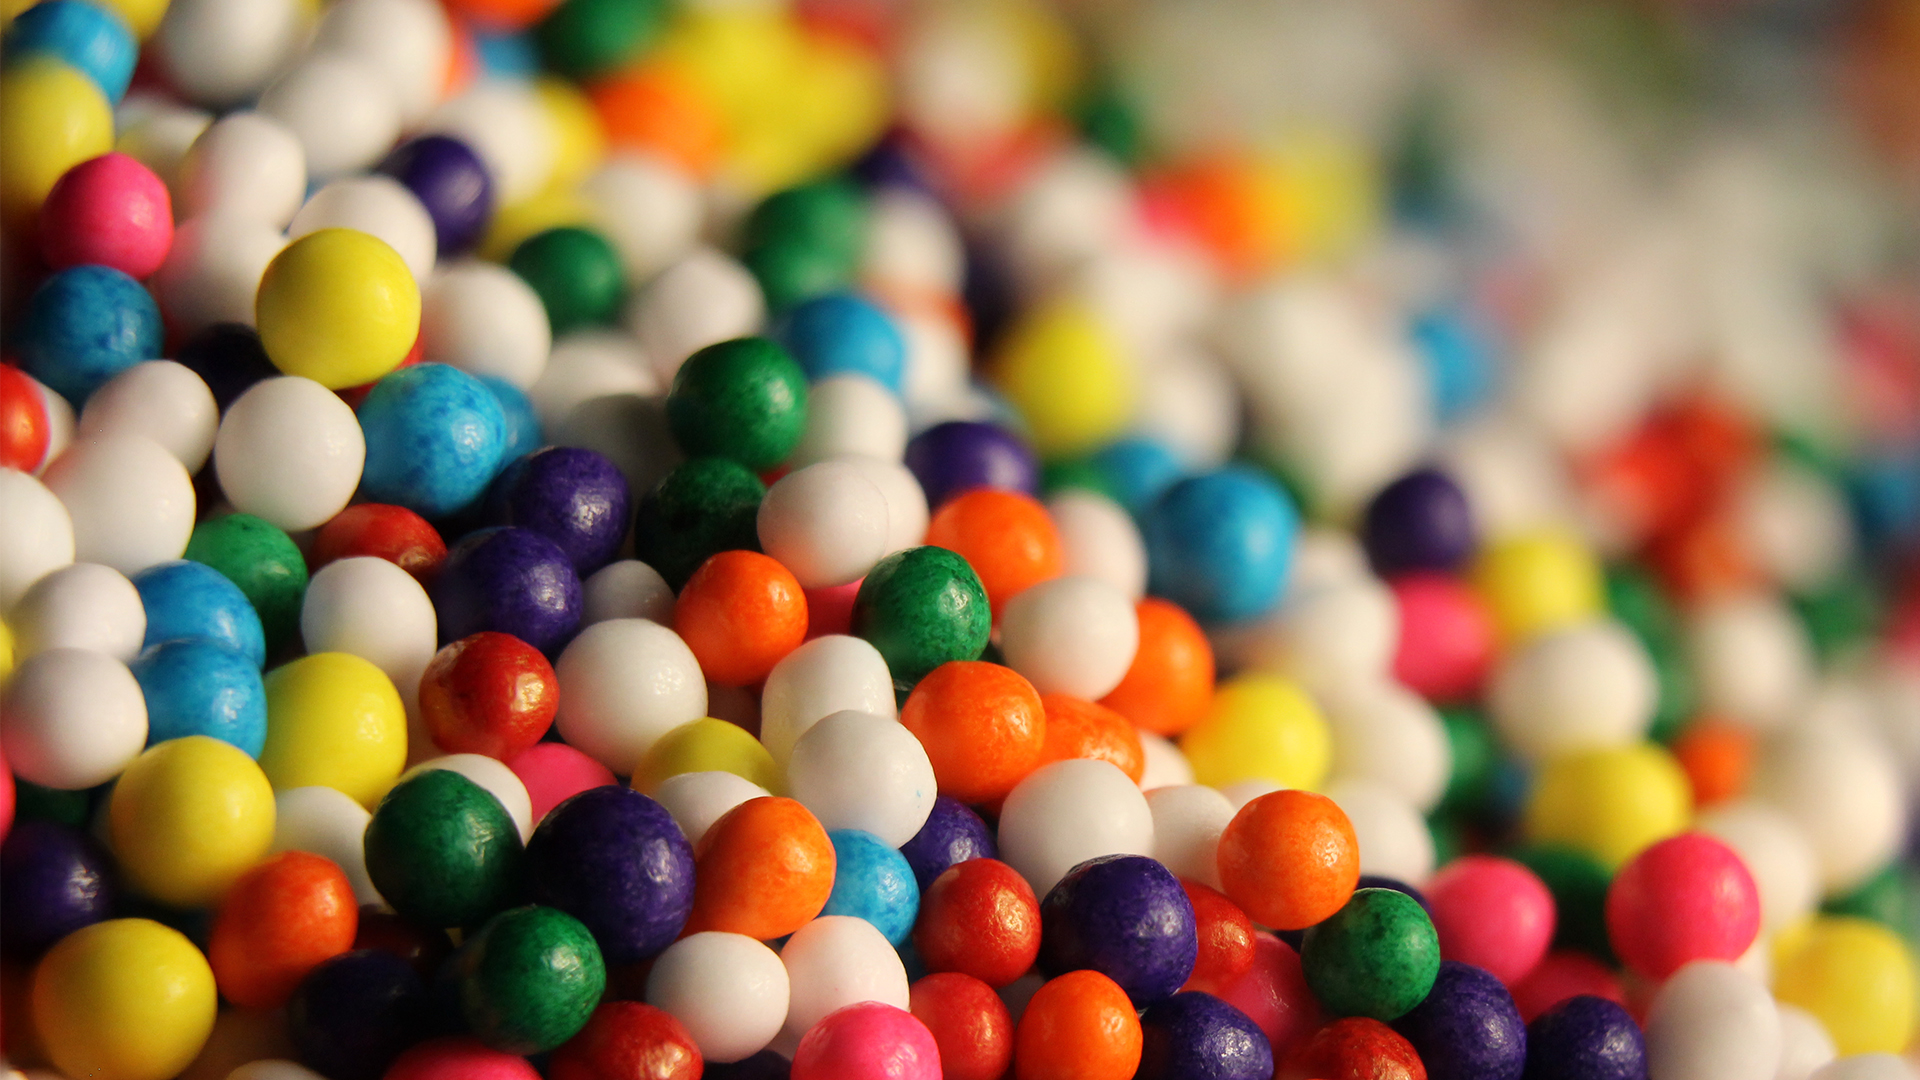
\includegraphics[width=100mm]{./figures/figure_example1.jpg}
    \caption{图片测试(最小宽度)\\Image test (Minimal width)}
  \end{figure}

\begin{figure}[H]
    \centering
    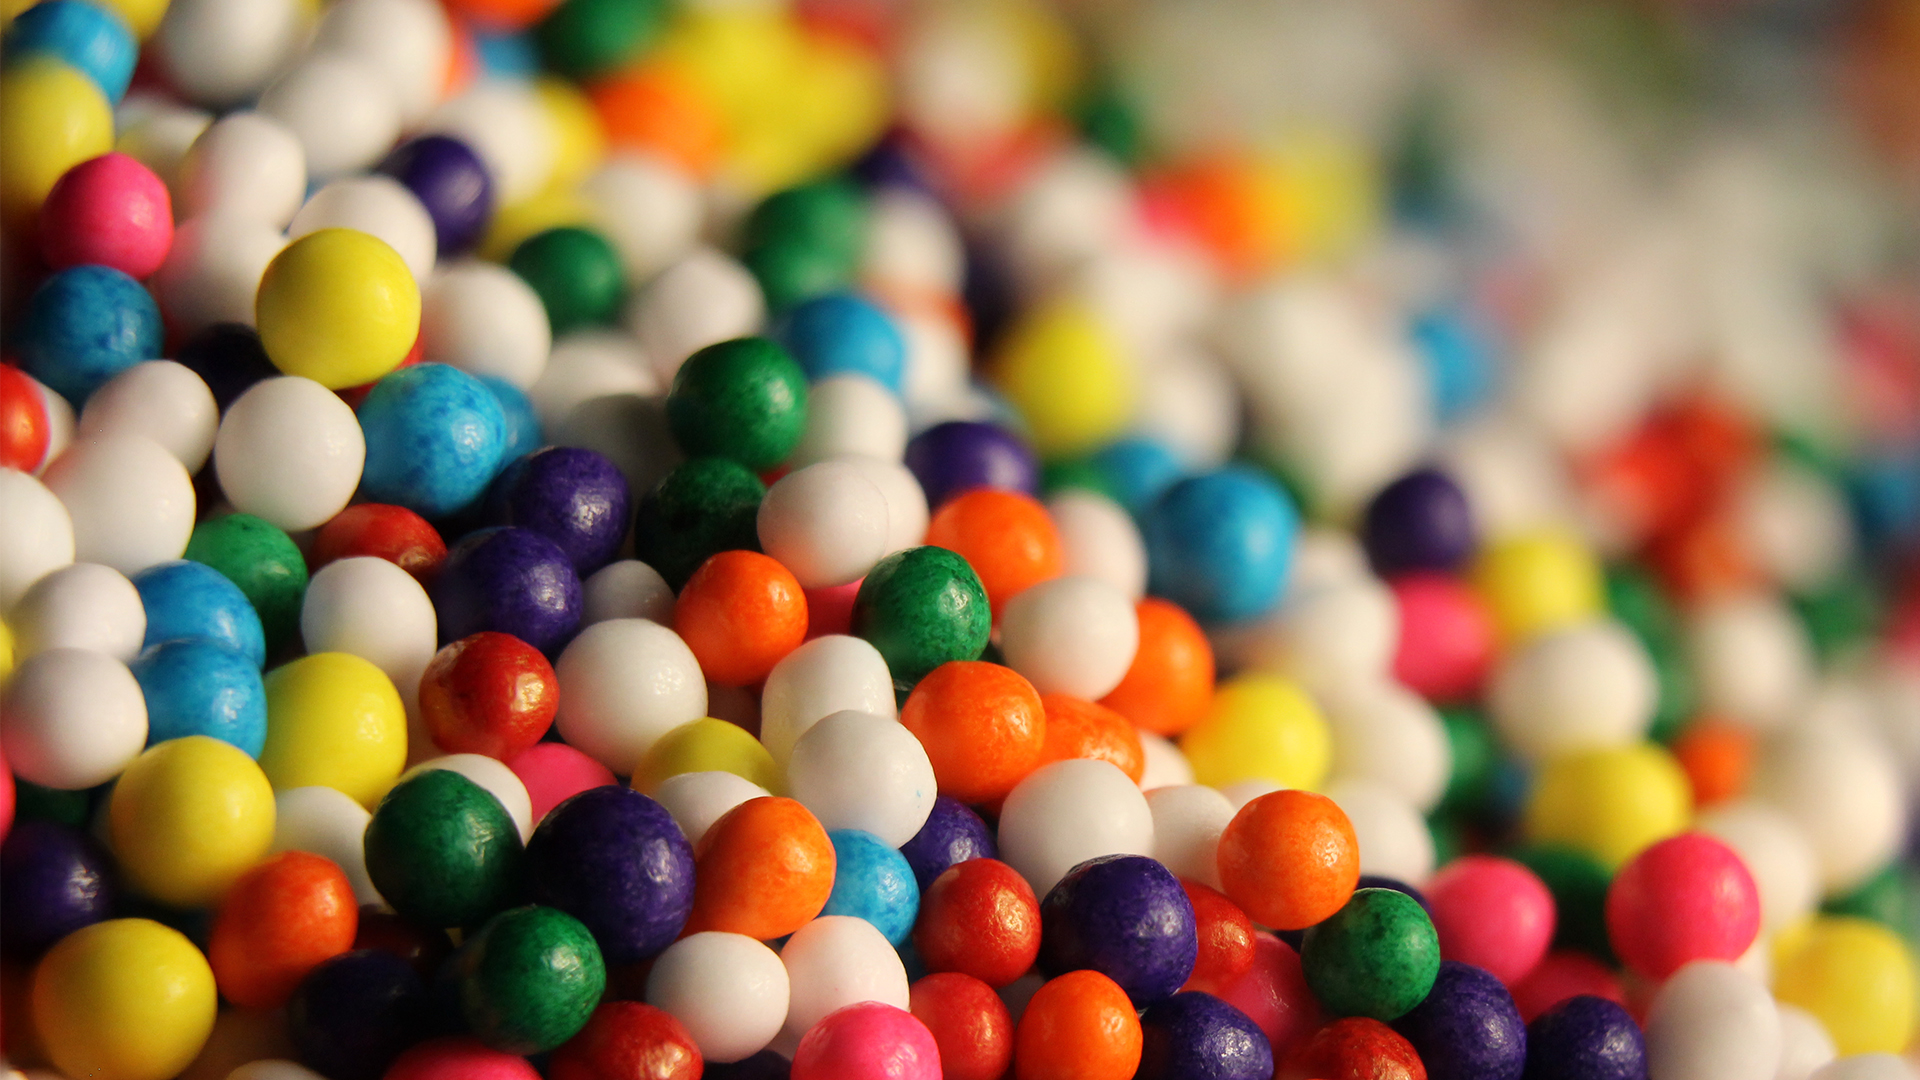
\includegraphics[width=130mm]{./figures/figure_example1.jpg}
    \caption{图片测试(最大宽度)\\Image test (Maximal width)}
\end{figure}
\par 注意:这里为了减少图片上下的空白,使用了float宏包。 %正文第四章                  % 
\section{注释与引用}这节用来展示注释与引用。

\subsection{注释——脚注与尾注}
\subsubsection{脚注}
\par 这里是脚注测试\footnote{1111111111}这里是脚注测试这里是脚注测试这里是脚注测试\footnote{2222222222}这里是脚注测试这里是脚注测试这里是脚注测试这里是脚注测试这里是脚注测试这里是脚注测试这里是脚注测试这里是脚注测试这里是脚注测试这里是脚注测试这里是脚注测试这里是脚注测试这里是脚注测试这里是脚注测试这里是脚注测试\footnote{3333333333}这里是脚注测试这里是脚注测试这里是脚注测试这里是脚注测试这里是脚注测试这里是脚注测试这里是脚注测试这里是脚注测试这里是脚注测试这里是脚注测试这里是脚注测试这里是脚注测试

\textcolor{red}{\textbf{\uline{注意!正如这份演示中所出现的情况,若该页(也就是本文档中的前一页)剩余空间不大,不足以显示足够多的文档与脚注,那么该段文字就会被移至下一页而留下空白。目前我们尚未找到解决的方法,所以如果遇到了这个问题,请修改排版,以留下足够大的空间。}}}

\subsubsection{尾注}
\par 这里是尾注测试\endnote{伴随着互联网的发展以及新的网络应用的出现,互联网用户由单纯的“读”网页,向“读、写”网页,共同建设互联网发展,由此网上产生了大量带有用户主观感情的数据,从这些带...}这里是尾注测试这里是尾注测试这里是尾注测试这里是尾注测试\endnote{尾注测试2}这里是尾注测试这里是尾注测试这里是尾注测试这里是尾注测试这里是尾注测试这里是尾注测试这里是尾注测试这里是尾注测试这里是尾注测试这里是尾注测试这里是尾注测试这里是尾注测试这里是尾注测试这里是尾注测试这里是尾注测试\endnote{尾注测试3}这里是尾注测试这里是尾注测试这里是尾注测试这里是尾注测试这里是尾注测试这里是尾注测试这里是尾注测试这里是尾注测试这里是尾注测试

\par \textcolor{red}{\textbf{\uline{注意!endnotes宏包并不支持hyperref,也就是无法通过点击文中尾注标号以跳转到尾注。当然,这在打印出来的文档中并不会造成任何影响。}}}
\par \textcolor{blue}{\textbf{\uline{提示:尾注出现在全文最后。为了区分脚注与尾注的编号,我们在尾注编号前加上了“尾注”二字。}}}

\subsection{文献引用的演示}
\par 本模板使用biblatex进行文献管理,这是一套相对较新的系统。另外,使用了hushidong制作的符合gb7714-2015标准的biblatex样式。在此对他的工作表示感谢,要完成这样的样式非常不容易。本模板中gb7714-2015.bbx与gb7714-2015.cbx即为他的作品,在这里打包发布以便使用。
\par 默认的bib文件位于~/reference/thesis-ref.bib,内容是由Wang Tianshu制作,在此仅作演示之用。关于bib文件的编写与管理请自行查找相关教程。
\par 下方的演示已经给出了正文中引用文献的基本方法,这与传统的cite命令是类似的。如有更多需求,请至\url{https://github.com/hushidong/biblatex-gb7714-2015}查找相关资料。
\par 文献\parencite{Yang_Hy200215}中提到xxxxxxx。
\par 文献\parencite{Joa1999}中提到yyyyyyy。
\par 文献\parencite{Altman1997}中提到zzzzzzz。
\par \textcolor{blue}{\textbf{\uline{本模板推荐使用parencite而不是cite命令,因为这样能与脚注所产生编号进行区分。}}}

 %正文第五章                  % 
                                                        %
%%%%%%%%%%%%%%%%%%%%%%%%%%%%%%%%%%%%%%%%%%%%%%%%%%%%%%%%%

\theendnotes %尾注

\cleardoublepage                                      %
\phantomsection                                       %生成参考文献
\addcontentsline{toc}{section}{参考文献}               %
\printbibliography[title={\heiti \zihao {-4}参考文献}] %

\clearpage                                       %
\begin{appendices}                               %
\renewcommand{\thesection}{\chinese{section}、}  %生成附录
%********************************************************************
% Appendix
%*******************************************************
% If problems with the headers: get headings in appendix etc. right
\markboth{\spacedlowsmallcaps{Appendix}}{\spacedlowsmallcaps{Appendix}}
%************************************************
\chapter{Appendix example}

\begin{flushright}{\slshape    
    We have seen that computer programming is an art, \\ 
    because it applies accumulated knowledge to the world, \\ 
    because it requires skill and ingenuity, and especially \\
    because it produces objects of beauty.} \\ \medskip
    --- \citeauthor{knuth:1974}, \citetitle{knuth:1974},
\citeyear{knuth:1974} 
\end{flushright}

\section{The \texttt{listings} package to include source code}
Source code is usually not part of the text of a thesis, but if it is an original contribution it makes sense to le the code speak by itself instead of describing it. The package \verb!listings! provide the proper layout tools. Refer to its manual if you need to use it, an example is given in listing \ref{lst:probCounter}.

\lstinputlisting[
	firstline=1,
	lastline=47,
	float=tb,
	language=C++,
	tabsize=2,
	numbers=left,
	numberstyle=\tiny,
	stepnumber=2,
	numbersep=5pt,
	caption={Code snippet with the recursive function to evaluate the pdf of the sum $Z_N$ of $N$ random variables equal to $X$.}, 
	captionpos=t,
	label=lst:probCounter
	]{CodeFiles/probabilityCounter.cpp}                    %
\end{appendices}                                 %

\clearpage                           %生成感谢
% ************************** Thesis Acknowledgements **************************

\begin{acknowledgements}      

For what has been an incredibly rewarding and wonderfully challenging 45 months I have several people to thank, several times over. David, for being a superb supervisor, whose unstinting zen and benevolent wisdom are a template for academic mentorship. Richard and Will, who both played the role of unofficial supervisors and always left their doors ajar. Sharon, whose gravitational pull kept me (and everyone else) in orbit. Dan, Mick and John for providing valuable advice along the way. Steve and Bill who as panel members took a much appreciated interest in my progression. Cam who provided valuable insights into my original project proposal. Various other fantastic UNSW folk that have contributed to the fun, including in no particular order: Sam, Sylvia, Eve, Mitch, Nick, Evan, Jo, Chris, Ben, Anna, Chantel, Francis, David and the Ecostats crew, Angela, Haba, Rhiannnon and the rest of the Big Ecology lab. The brilliant academics of the UCT Botany Dept, and in particular Jeremy and Tony who as honours supervisors made me think differently, in a really good way. My patient parents who have supported me unconditionally in my every pursuit. My generous brother who amongst many other things has done his best to keep me in fashion. My wonderful wife Shan, a mention in the acknowledgements of my thesis almost makes a mockery of your contribution; you rock like Kilimanjaro. Finally, I thank my amazing little Ash Mae, who makes me stop and smell the roses (and the nappies).


\end{acknowledgements}
 %

\end{document}